% Options for packages loaded elsewhere
\PassOptionsToPackage{unicode}{hyperref}
\PassOptionsToPackage{hyphens}{url}
%
\documentclass[
]{article}
\usepackage{amsmath,amssymb}
\usepackage{lmodern}
\usepackage{iftex}
\ifPDFTeX
  \usepackage[T1]{fontenc}
  \usepackage[utf8]{inputenc}
  \usepackage{textcomp} % provide euro and other symbols
\else % if luatex or xetex
  \usepackage{unicode-math}
  \defaultfontfeatures{Scale=MatchLowercase}
  \defaultfontfeatures[\rmfamily]{Ligatures=TeX,Scale=1}
\fi
% Use upquote if available, for straight quotes in verbatim environments
\IfFileExists{upquote.sty}{\usepackage{upquote}}{}
\IfFileExists{microtype.sty}{% use microtype if available
  \usepackage[]{microtype}
  \UseMicrotypeSet[protrusion]{basicmath} % disable protrusion for tt fonts
}{}
\makeatletter
\@ifundefined{KOMAClassName}{% if non-KOMA class
  \IfFileExists{parskip.sty}{%
    \usepackage{parskip}
  }{% else
    \setlength{\parindent}{0pt}
    \setlength{\parskip}{6pt plus 2pt minus 1pt}}
}{% if KOMA class
  \KOMAoptions{parskip=half}}
\makeatother
\usepackage{xcolor}
\usepackage[margin=1in]{geometry}
\usepackage{graphicx}
\makeatletter
\def\maxwidth{\ifdim\Gin@nat@width>\linewidth\linewidth\else\Gin@nat@width\fi}
\def\maxheight{\ifdim\Gin@nat@height>\textheight\textheight\else\Gin@nat@height\fi}
\makeatother
% Scale images if necessary, so that they will not overflow the page
% margins by default, and it is still possible to overwrite the defaults
% using explicit options in \includegraphics[width, height, ...]{}
\setkeys{Gin}{width=\maxwidth,height=\maxheight,keepaspectratio}
% Set default figure placement to htbp
\makeatletter
\def\fps@figure{htbp}
\makeatother
\setlength{\emergencystretch}{3em} % prevent overfull lines
\providecommand{\tightlist}{%
  \setlength{\itemsep}{0pt}\setlength{\parskip}{0pt}}
\setcounter{secnumdepth}{-\maxdimen} % remove section numbering
\usepackage{fontspec}
\usepackage{polyglossia}
\setmainlanguage[babelshorthands=true]{german}
\setmainfont{merriweather}
\setsansfont{Montserrat}
\geometry{vmargin=1in,hmargin=1.25in}
\usepackage{xcolor}
\usepackage{titlesec}
\definecolor{Blue}{HTML}{2F5496}
\titleformat{\section}{\Large\sffamily\color{Blue}}{}{0pt}{}
\titleformat{\subsection}{\large\sffamily\color{Blue}}{}{0pt}{}
\titlespacing\section{0pt}{24pt plus 4pt minus 2pt}{6pt plus 2pt minus 2pt}
\titlespacing\subsection{0pt}{12pt plus 4pt minus 2pt}{2pt plus 2pt minus 2pt}
\usepackage{parskip}
\usepackage{booktabs}
\usepackage{longtable}
\usepackage{array}
\usepackage{multirow}
\usepackage{wrapfig}
\usepackage{float}
\usepackage{colortbl}
\usepackage{pdflscape}
\usepackage{tabu}
\usepackage{threeparttable}
\usepackage{threeparttablex}
\usepackage[normalem]{ulem}
\usepackage{makecell}
\usepackage{xcolor}
\usepackage{siunitx}
\newcolumntype{d}{S[input-symbols = ()]}
\ifLuaTeX
  \usepackage{selnolig}  % disable illegal ligatures
\fi
\IfFileExists{bookmark.sty}{\usepackage{bookmark}}{\usepackage{hyperref}}
\IfFileExists{xurl.sty}{\usepackage{xurl}}{} % add URL line breaks if available
\urlstyle{same} % disable monospaced font for URLs
\hypersetup{
  pdftitle={Example},
  pdfauthor={Nixon Candiales},
  hidelinks,
  pdfcreator={LaTeX via pandoc}}

\title{Example}
\author{Nixon Candiales}
\date{\today}

\begin{document}
\maketitle

\hypertarget{part-1}{%
\section{Part 1}\label{part-1}}

\hypertarget{whats-the-answer-to-life-the-universe-and-everything}{%
\subsection{whats the answer to life the universe and
everything?}\label{whats-the-answer-to-life-the-universe-and-everything}}

Lorem ipsum\ldots{}

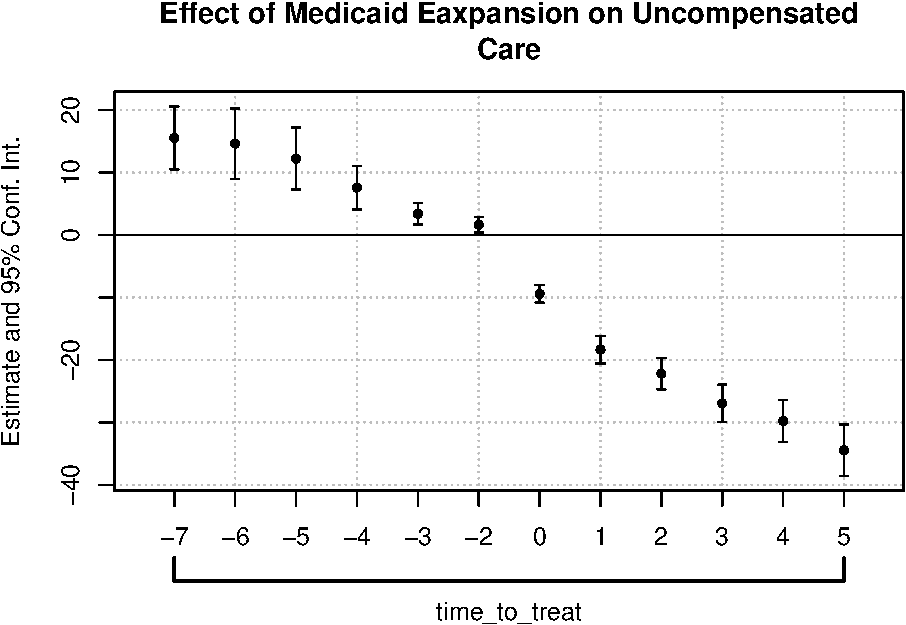
\includegraphics{Report_files/figure-latex/Figures-1.pdf}
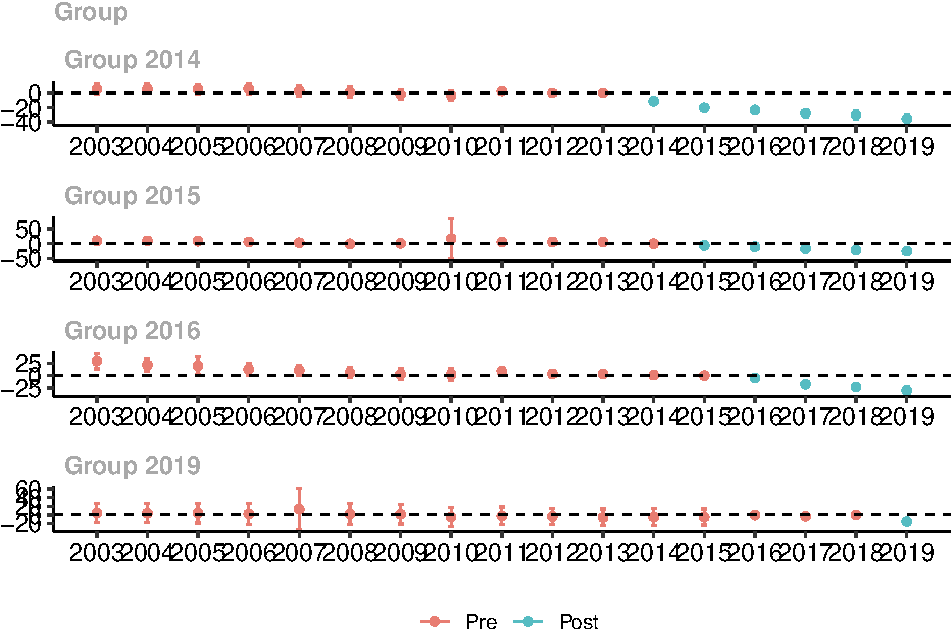
\includegraphics{Report_files/figure-latex/Figures-2.pdf}

\begin{verbatim}
FALSE `geom_smooth()` using method = 'loess' and formula 'y ~ x'
\end{verbatim}

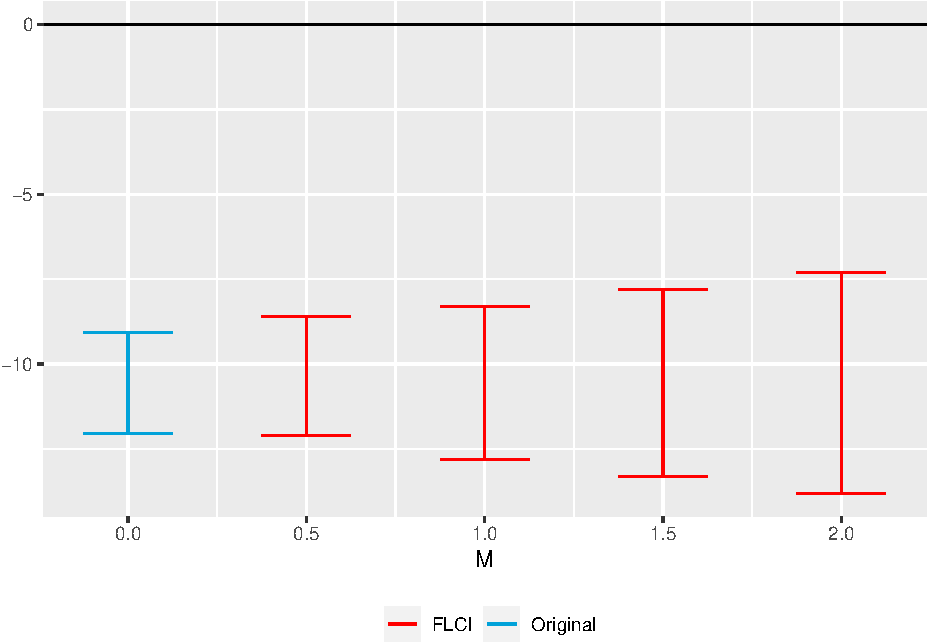
\includegraphics{Report_files/figure-latex/Figures-3.pdf}
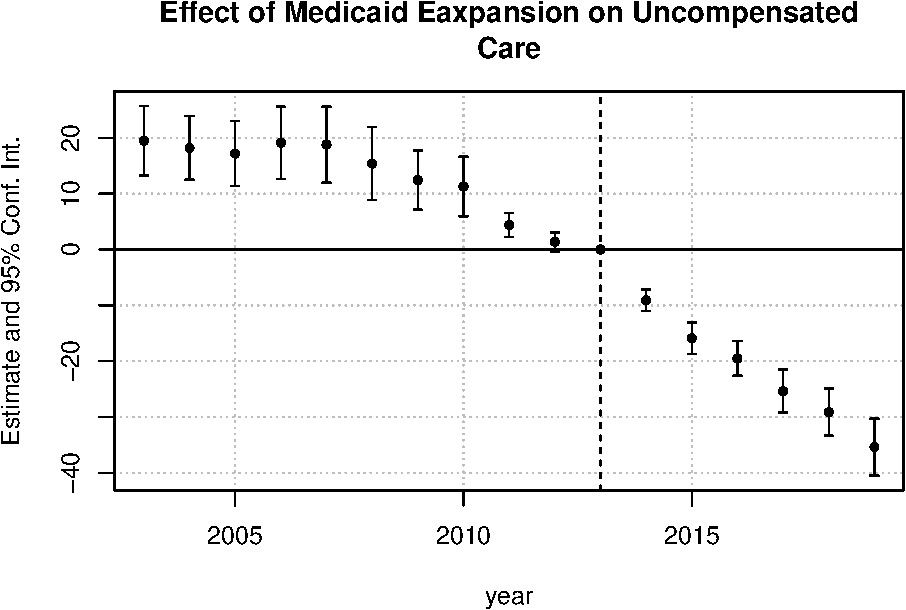
\includegraphics{Report_files/figure-latex/Figures-4.pdf}
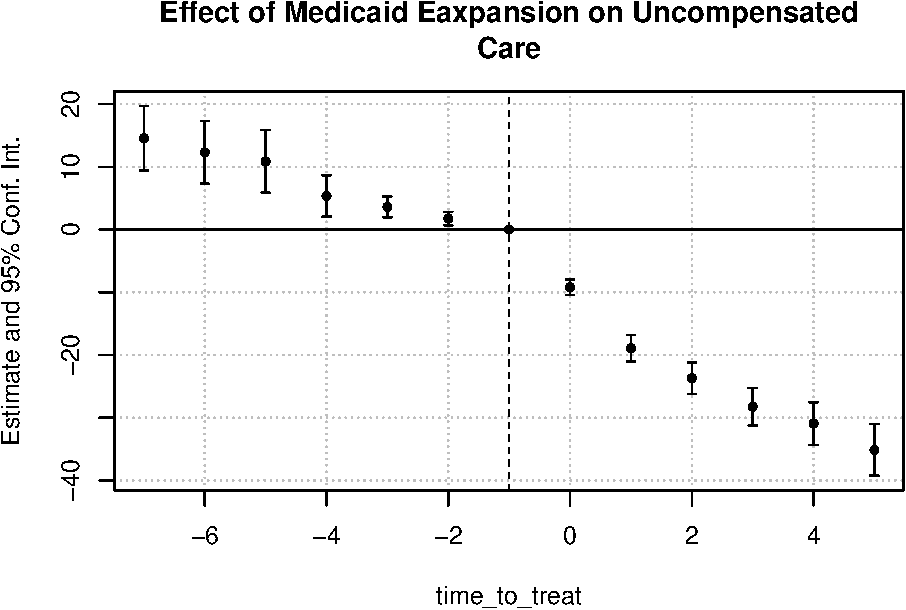
\includegraphics{Report_files/figure-latex/Figures-5.pdf}
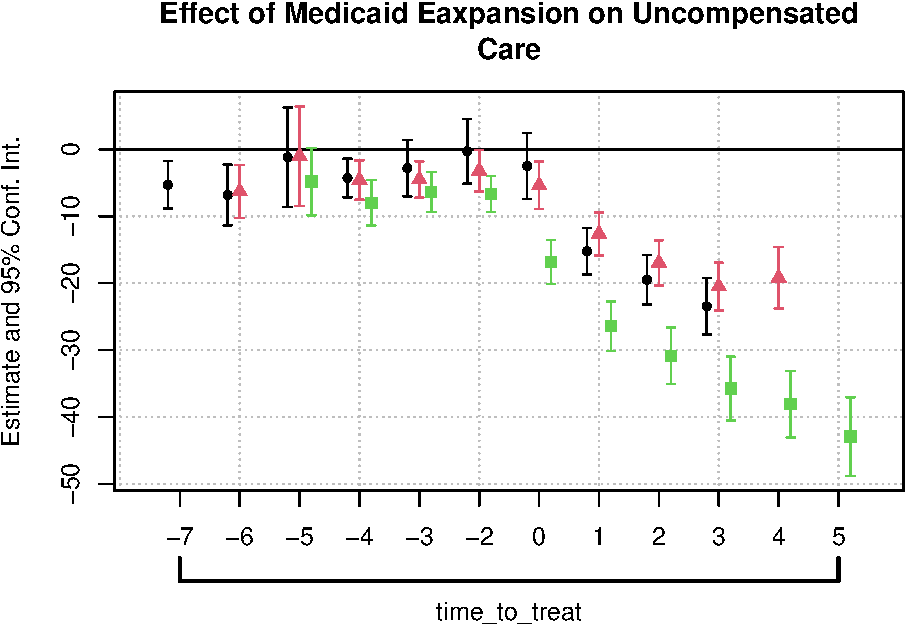
\includegraphics{Report_files/figure-latex/Figures-6.pdf}
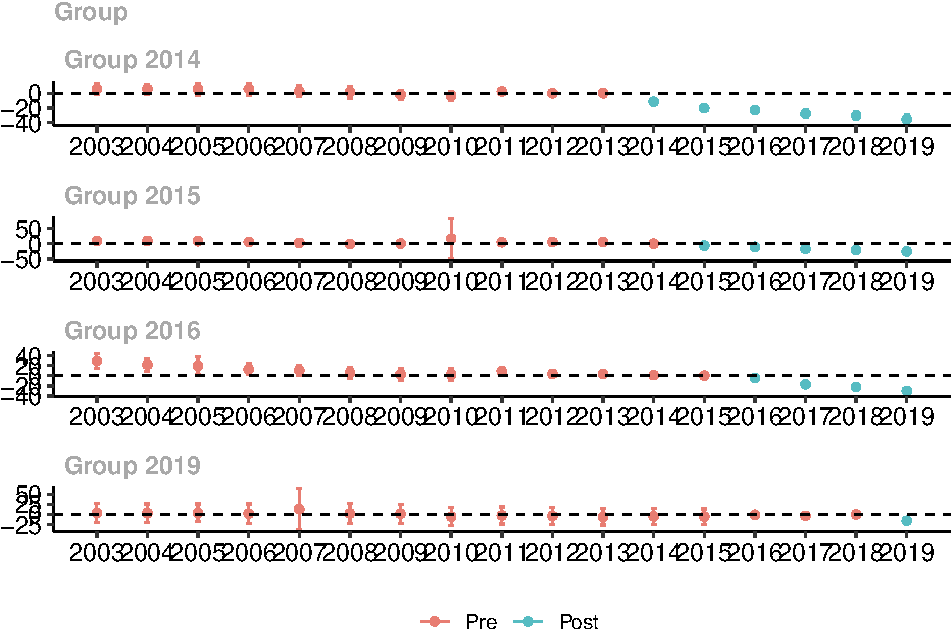
\includegraphics{Report_files/figure-latex/Figures-7.pdf}
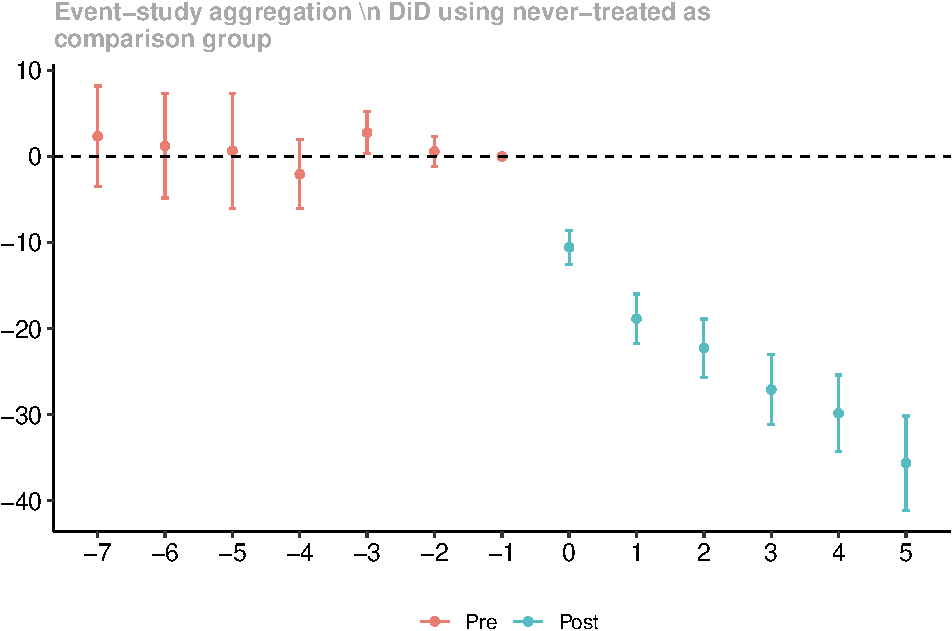
\includegraphics{Report_files/figure-latex/Figures-8.pdf}
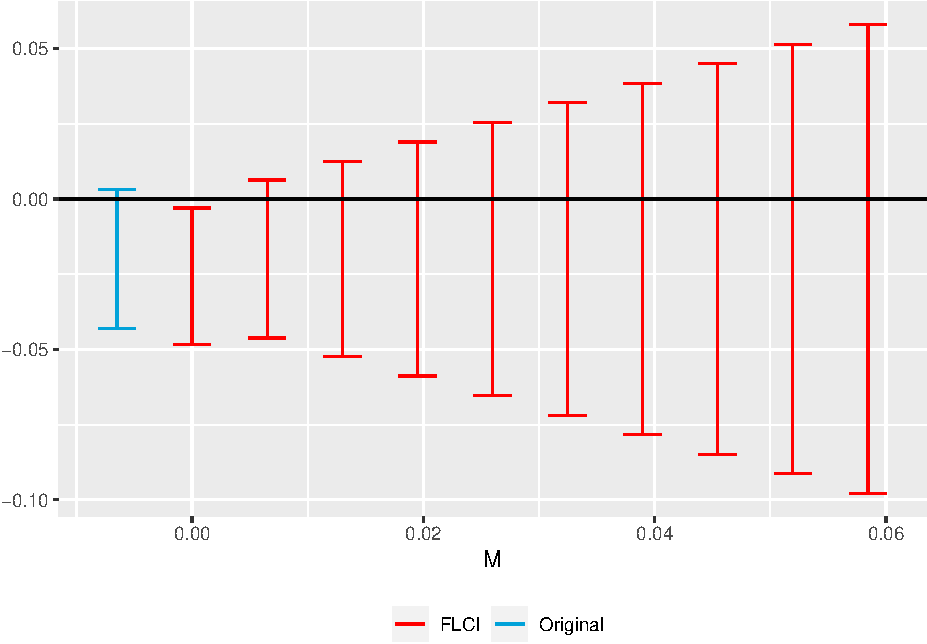
\includegraphics{Report_files/figure-latex/Figures-9.pdf}
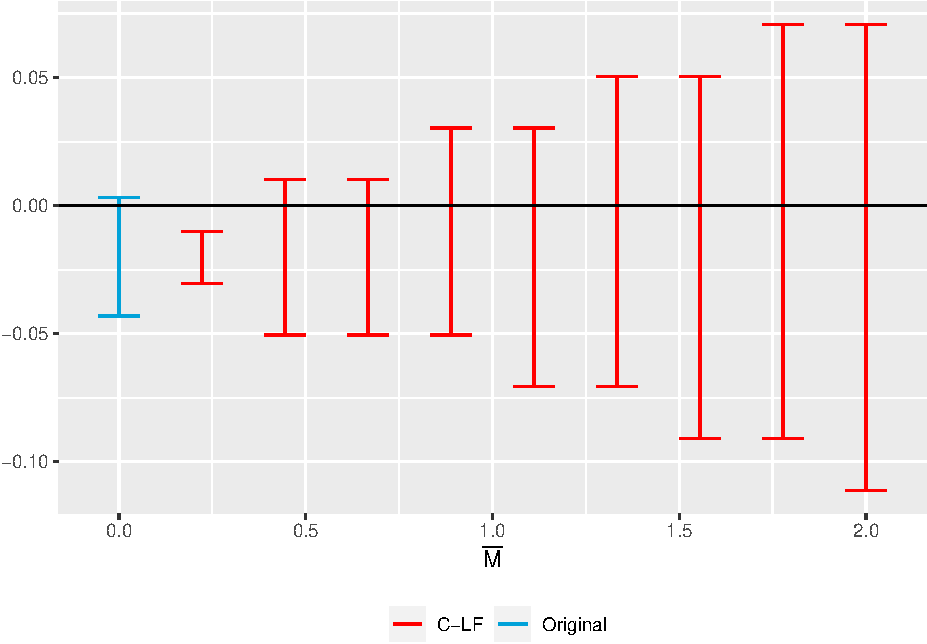
\includegraphics{Report_files/figure-latex/Figures-10.pdf} \% latex
table generated in R 4.2.1 by xtable 1.8-4 package \% Wed Sep 21
04:41:04 2022

\begin{table}[ht]
\centering
\begin{tabular}{rrrrrr}
  \hline
 & year & mean & sd & min & max \\ 
  \hline
1 & 2003 & 13.26 & 30.68 & 0.00 & 777.99 \\ 
  2 & 2004 & 15.16 & 37.51 & 0.00 & 820.25 \\ 
  3 & 2005 & 17.31 & 39.89 & 0.00 & 939.13 \\ 
  4 & 2006 & 20.53 & 49.09 & 0.00 & 1074.62 \\ 
  5 & 2007 & 22.85 & 52.29 & 0.00 & 1203.37 \\ 
  6 & 2008 & 25.81 & 58.58 & 0.00 & 1361.81 \\ 
  7 & 2009 & 26.51 & 44.88 & 0.00 & 583.98 \\ 
  8 & 2010 & 28.59 & 67.33 & 0.00 & 2793.92 \\ 
  9 & 2011 & 25.19 & 59.22 & 0.00 & 2059.70 \\ 
  10 & 2012 & 28.01 & 67.71 & 0.00 & 1882.62 \\ 
  11 & 2013 & 30.20 & 68.94 & 0.00 & 1652.58 \\ 
  12 & 2014 & 30.32 & 74.00 & 0.00 & 2024.85 \\ 
  13 & 2015 & 28.59 & 71.72 & 0.00 & 2054.15 \\ 
  14 & 2016 & 29.83 & 77.46 & 0.00 & 2390.67 \\ 
  15 & 2017 & 32.08 & 84.52 & 0.00 & 2733.60 \\ 
  16 & 2018 & 34.71 & 88.23 & 0.00 & 2606.35 \\ 
  17 & 2019 & 38.61 & 97.94 & 0.00 & 2648.26 \\ 
   \hline
\end{tabular}
\end{table}

\% latex table generated in R 4.2.1 by xtable 1.8-4 package \% Wed Sep
21 04:41:04 2022

\begin{table}[ht]
\centering
\begin{tabular}{rrrrrr}
  \hline
 & year & mean & sd & min & max \\ 
  \hline
1 & 2003 & 284.13 & 383.61 & 1.66 & 4722.76 \\ 
  2 & 2004 & 316.73 & 430.15 & 0.27 & 5525.73 \\ 
  3 & 2005 & 364.92 & 495.20 & 1.14 & 6398.55 \\ 
  4 & 2006 & 415.73 & 540.60 & 1.33 & 6718.17 \\ 
  5 & 2007 & 462.17 & 622.69 & 0.99 & 8577.05 \\ 
  6 & 2008 & 492.36 & 634.20 & 0.97 & 7743.08 \\ 
  7 & 2009 & 527.15 & 687.54 & 0.89 & 9139.32 \\ 
  8 & 2010 & 548.93 & 749.12 & 0.84 & 9857.53 \\ 
  9 & 2011 & 450.57 & 744.13 & -27.58 & 10572.29 \\ 
  10 & 2012 & 474.12 & 796.22 & 0.85 & 11865.32 \\ 
  11 & 2013 & 507.36 & 869.11 & 0.95 & 12751.71 \\ 
  12 & 2014 & 544.79 & 950.09 & 1.09 & 13376.35 \\ 
  13 & 2015 & 588.96 & 1013.40 & 1.05 & 14143.53 \\ 
  14 & 2016 & 641.25 & 1118.92 & -177.03 & 15618.75 \\ 
  15 & 2017 & 689.44 & 1220.60 & 1.00 & 16863.43 \\ 
  16 & 2018 & 743.16 & 1341.17 & 1.07 & 18677.25 \\ 
  17 & 2019 & 814.39 & 1488.68 & 0.72 & 22000.93 \\ 
   \hline
\end{tabular}
\end{table}

\begin{table}[H] \centering 
  \caption{Regression table with stargazer} 
  \label{tab2} 
\begin{tabular}{@{\extracolsep{5pt}}lcccc} 
\\[-1.8ex]\hline 
\hline \\[-1.8ex] 
 & \multicolumn{4}{c}{\textit{Dependent variable:}} \\ 
\cline{2-5} 
\\[-1.8ex] & \multicolumn{4}{c}{unc\_care} \\ 
 & M1 & M2 & M3 &  \\ 
\hline \\[-1.8ex] 
 Treatment & $-$28.191$^{***}$ & $-$26.243$^{***}$ & $-$12.003$^{***}$ & $-$12.424$^{***}$ \\ 
  & (1.883) & (1.795) & (1.811) & (1.543) \\ 
  & & & & \\ 
\hline \\[-1.8ex] 
Observations & 79,557 & 79,557 & 79,557 & 79,557 \\ 
R$^{2}$ & 0.699 & 0.697 & 0.690 & 0.690 \\ 
Adjusted R$^{2}$ & 0.675 & 0.673 & 0.665 & 0.665 \\ 
Residual Std. Error (df = 73725) & 39.701 & 39.829 & 40.304 & 40.313 \\ 
\hline 
\hline \\[-1.8ex] 
\textit{Note:}  & \multicolumn{4}{r}{$^{*}$p$<$0.1; $^{**}$p$<$0.05; $^{***}$p$<$0.01} \\ 
\end{tabular} 
\end{table}

\begin{table}

\caption{\label{tab:table-4}Regression table with stargazer}
\centering
\begin{tabular}[t]{lcccc}
\toprule
  & d & d\_14 & d\_15 & d\_16\\
\midrule
Treatment & \num{-28.191}*** & \num{-26.243}*** & \num{-12.003}*** & \num{-12.424}***\\
 & (\num{1.883}) & (\num{1.795}) & (\num{1.811}) & (\num{1.543})\\
\midrule
Num.Obs. & \num{79557} & \num{79557} & \num{79557} & \num{79557}\\
R2 & \num{0.699} & \num{0.697} & \num{0.690} & \num{0.690}\\
R2 Adj. & \num{0.675} & \num{0.673} & \num{0.665} & \num{0.665}\\
AIC & \num{817139.6} & \num{817654.2} & \num{819537.5} & \num{819575.0}\\
BIC & \num{871294.5} & \num{871809.1} & \num{873692.4} & \num{873729.9}\\
RMSE & \num{38.22} & \num{38.34} & \num{38.80} & \num{38.81}\\
Std.Errors & by: pn & by: pn & by: pn & by: pn\\
\bottomrule
\multicolumn{5}{l}{\rule{0pt}{1em}+ p $<$ 0.1, * p $<$ 0.05, ** p $<$ 0.01, *** p $<$ 0.001}\\
\end{tabular}
\end{table}

\begin{table}

\caption{\label{tab:table-4}Regression table with stargazer}
\centering
\begin{tabular}[t]{lc}
\toprule
  & Model 1\\
\midrule
year = 2003 × treated & \num{19.485}***\\
 & (\num{3.164})\\
year = 2004 × treated & \num{18.189}***\\
 & (\num{2.908})\\
year = 2005 × treated & \num{17.172}***\\
 & (\num{2.965})\\
year = 2006 × treated & \num{19.119}***\\
 & (\num{3.292})\\
year = 2007 × treated & \num{18.782}***\\
 & (\num{3.478})\\
year = 2008 × treated & \num{15.392}***\\
 & (\num{3.328})\\
year = 2009 × treated & \num{12.430}***\\
 & (\num{2.711})\\
year = 2010 × treated & \num{11.285}***\\
 & (\num{2.717})\\
year = 2011 × treated & \num{4.376}***\\
 & (\num{1.106})\\
year = 2012 × treated & \num{1.371}\\
 & (\num{0.873})\\
year = 2014 × treated & \num{-9.102}***\\
 & (\num{0.987})\\
year = 2015 × treated & \num{-15.893}***\\
 & (\num{1.431})\\
year = 2016 × treated & \num{-19.503}***\\
 & (\num{1.585})\\
year = 2017 × treated & \num{-25.378}***\\
 & (\num{1.959})\\
year = 2018 × treated & \num{-29.139}***\\
 & (\num{2.155})\\
year = 2019 × treated & \num{-35.394}***\\
 & (\num{2.603})\\
\midrule
Num.Obs. & \num{79557}\\
AIC & \num{804621.4}\\
BIC & \num{804779.2}\\
RMSE & \num{38.01}\\
Std.Errors & by: pn\\
FE: pn & X\\
FE: year & X\\
\bottomrule
\multicolumn{2}{l}{\rule{0pt}{1em}+ p $<$ 0.1, * p $<$ 0.05, ** p $<$ 0.01, *** p $<$ 0.001}\\
\end{tabular}
\end{table}

\begin{table}

\caption{\label{tab:table-4}Regression table with stargazer}
\centering
\begin{tabular}[t]{lc}
\toprule
  & Model 1\\
\midrule
time\_to\_treat = -7 × treated & \num{5.137}***\\
 & (\num{1.412})\\
time\_to\_treat = -6 × treated & \num{4.920}**\\
 & (\num{1.502})\\
time\_to\_treat = -5 × treated & \num{2.254}\\
 & (\num{1.551})\\
time\_to\_treat = -4 × treated & \num{-1.602}\\
 & (\num{1.308})\\
time\_to\_treat = -3 × treated & \num{-2.416}*\\
 & (\num{1.027})\\
time\_to\_treat = -2 × treated & \num{-0.141}\\
 & (\num{0.578})\\
time\_to\_treat = 0 × treated & \num{8.151}***\\
 & (\num{1.599})\\
time\_to\_treat = 1 × treated & \num{-16.830}***\\
 & (\num{1.009})\\
time\_to\_treat = 2 × treated & \num{-22.370}***\\
 & (\num{1.256})\\
time\_to\_treat = 3 × treated & \num{-27.793}***\\
 & (\num{1.537})\\
time\_to\_treat = 4 × treated & \num{-30.231}***\\
 & (\num{1.738})\\
time\_to\_treat = 5 × treated & \num{-33.524}***\\
 & (\num{2.060})\\
\midrule
Num.Obs. & \num{79557}\\
AIC & \num{805085.8}\\
BIC & \num{805206.5}\\
RMSE & \num{38.12}\\
Std.Errors & by: pn\\
FE: pn & X\\
FE: year & X\\
\bottomrule
\multicolumn{2}{l}{\rule{0pt}{1em}+ p $<$ 0.1, * p $<$ 0.05, ** p $<$ 0.01, *** p $<$ 0.001}\\
\end{tabular}
\end{table}

\begin{table}

\caption{\label{tab:table-4}Regression table with stargazer}
\centering
\begin{tabular}[t]{lccc}
\toprule
  & mod.sa.2016 & mod.sa.2015 & mod.sa.2014\\
\midrule
time\_to\_treat = -7 & \num{-5.298}** &  & \\
 & (\num{1.806}) &  & \\
time\_to\_treat = -6 & \num{-6.820}** & \num{-6.301}** & \\
 & (\num{2.306}) & (\num{2.025}) & \\
time\_to\_treat = -5 & \num{-1.181} & \num{-1.023} & \num{-4.815}+\\
 & (\num{3.792}) & (\num{3.790}) & (\num{2.575})\\
time\_to\_treat = -4 & \num{-4.281}** & \num{-4.591}** & \num{-7.985}***\\
 & (\num{1.474}) & (\num{5.908}) & (\num{1.733})\\
time\_to\_treat = -3 & \num{-2.801} & \num{-4.501}** & \num{-6.371}***\\
 & (\num{2.155}) & (\num{2.097}) & (\num{1.529})\\
time\_to\_treat = -2 & \num{-0.286} & \num{-3.207}* & \num{-6.684}***\\
 & (\num{2.473}) & (\num{1.384}) & (\num{1.369})\\
time\_to\_treat = 0 & \num{-2.493} & \num{-5.394}** & \num{-16.855}***\\
 & (\num{2.524}) & (\num{1.278}) & (\num{1.673})\\
time\_to\_treat = 1 & \num{-15.240}*** & \num{-12.623}*** & \num{-26.405}***\\
 & (\num{1.783}) & (\num{1.921}) & (\num{1.890})\\
time\_to\_treat = 2 & \num{-19.497}*** & \num{-16.957}*** & \num{-30.859}***\\
 & (\num{1.880}) & (\num{2.156}) & (\num{2.158})\\
time\_to\_treat = 3 & \num{-23.461}*** & \num{-20.513}*** & \num{-35.758}***\\
 & (\num{2.161}) & (\num{2.128}) & (\num{2.431})\\
time\_to\_treat = 4 &  & \num{-19.194}*** & \num{-38.103}***\\
 &  & (\num{5.484}) & (\num{2.538})\\
time\_to\_treat = 5 &  &  & \num{-42.934}***\\
 &  &  & (\num{3.003})\\
\midrule
Num.Obs. & \num{79557} & \num{79557} & \num{79557}\\
AIC & \num{807862.7} & \num{807729.3} & \num{804897.4}\\
BIC & \num{807964.8} & \num{807831.4} & \num{804999.5}\\
RMSE & \num{38.79} & \num{38.76} & \num{38.07}\\
Std.Errors & by: pn & by: pn & by: pn\\
FE: pn & X & X & X\\
FE: year & X & X & X\\
\bottomrule
\multicolumn{4}{l}{\rule{0pt}{1em}+ p $<$ 0.1, * p $<$ 0.05, ** p $<$ 0.01, *** p $<$ 0.001}\\
\end{tabular}
\end{table}

\begin{table}

\caption{\label{tab:table-4}Regression table with stargazer}
\centering
\begin{tabular}[t]{lc}
\toprule
  & Model 1\\
\midrule
ATT(2014,2012) & \num{0.501}\\
 & (\num{0.921})\\
ATT(2014,2013) & \num{0.000}\\
ATT(2014,2014) & \num{-10.982}\\
 & (\num{2.353})\\
ATT(2014,2015) & \num{-19.827}\\
 & (\num{4.032})\\
ATT(2014,2016) & \num{-22.794}\\
 & (\num{4.423})\\
ATT(2014,2017) & \num{-27.690}\\
 & (\num{5.425})\\
ATT(2014,2018) & \num{-30.212}\\
 & (\num{6.527})\\
ATT(2014,2019) & \num{-35.792}\\
 & (\num{8.895})\\
ATT(2015,2012) & \num{6.244}\\
 & (\num{2.375})\\
ATT(2015,2013) & \num{5.781}\\
 & (\num{1.828})\\
ATT(2015,2014) & \num{0.000}\\
ATT(2015,2015) & \num{-5.401}\\
 & (\num{2.551})\\
ATT(2015,2016) & \num{-9.522}\\
 & (\num{2.280})\\
ATT(2015,2017) & \num{-16.522}\\
 & (\num{3.393})\\
ATT(2015,2018) & \num{-20.673}\\
 & (\num{4.413})\\
ATT(2015,2019) & \num{-25.534}\\
 & (\num{6.938})\\
ATT(2016,2012) & \num{3.523}\\
 & (\num{4.837})\\
ATT(2016,2013) & \num{2.544}\\
 & (\num{4.361})\\
ATT(2016,2014) & \num{0.879}\\
 & (\num{1.577})\\
ATT(2016,2015) & \num{0.000}\\
ATT(2016,2016) & \num{-4.752}\\
 & (\num{1.310})\\
ATT(2016,2017) & \num{-18.249}\\
 & (\num{4.502})\\
ATT(2016,2018) & \num{-23.546}\\
 & (\num{5.533})\\
ATT(2016,2019) & \num{-31.190}\\
 & (\num{6.930})\\
ATT(2019,2012) & \num{-2.711}\\
 & (\num{11.211})\\
ATT(2019,2013) & \num{-4.623}\\
 & (\num{10.933})\\
ATT(2019,2014) & \num{-3.978}\\
 & (\num{8.697})\\
ATT(2019,2015) & \num{-3.711}\\
 & (\num{6.632})\\
ATT(2019,2016) & \num{-0.441}\\
 & (\num{4.756})\\
ATT(2019,2017) & \num{-3.331}\\
 & (\num{3.440})\\
ATT(2019,2018) & \num{0.000}\\
ATT(2019,2019) & \num{-15.267}\\
 & (\num{3.530})\\
\midrule
Num.Obs. & \num{51}\\
Std.Errors & by: state\_id\\
ngroup & \num{4.000}\\
ntime & \num{8.000}\\
control.group & nevertreated\\
est.method & dr\\
\bottomrule
\end{tabular}
\end{table}

\begin{table}

\caption{\label{tab:table-4}Regression table with stargazer}
\centering
\begin{tabular}[t]{lc}
\toprule
  & Model 1\\
\midrule
ATT(-5) & \num{-3.978}\\
 & (\num{9.523})\\
ATT(-4) & \num{-0.094}\\
 & (\num{5.252})\\
ATT(-3) & \num{3.277}\\
 & (\num{3.020})\\
ATT(-2) & \num{0.764}\\
 & (\num{0.909})\\
ATT(-1) & \num{0.000}\\
ATT(0) & \num{-10.375}\\
 & (\num{2.164})\\
ATT(1) & \num{-18.762}\\
 & (\num{3.412})\\
ATT(2) & \num{-22.253}\\
 & (\num{4.043})\\
ATT(3) & \num{-27.251}\\
 & (\num{4.979})\\
ATT(4) & \num{-29.744}\\
 & (\num{6.487})\\
ATT(5) & \num{-35.792}\\
 & (\num{8.298})\\
\midrule
Num.Obs. & \num{51}\\
Std.Errors & by: state\_id\\
type & dynamic\\
ngroup & \num{4.000}\\
ntime & \num{8.000}\\
control.group & nevertreated\\
est.method & dr\\
\bottomrule
\end{tabular}
\end{table}

\end{document}
